\documentclass{standalone}
\usepackage{tikz}
\usepackage{amsmath}

\begin{document}
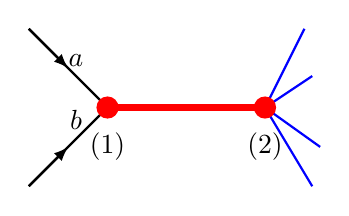
\begin{tikzpicture}
    \draw[-latex,thick] (-1,1)--(-0.5,0.5);
    \draw[-latex,thick] (-1,-1)--(-0.5,-0.5);
    \node[above] at(-0.4,0.4){$a$};
    \node[above] at(-0.4,-0.4){$b$};
    \draw[thick] (-1,1)--(0,0);
    \draw[thick] (-1,-1)--(0,0);
    \fill[red] (0,0) circle (4pt) node[black,yshift=-0.5cm] {$(1)$};
    \fill[red] (0,-0.05) rectangle (2,0.05);
    \draw[blue, thick] (2,0)--(2.5,1);
    \draw[blue, thick] (2,0)--(2.6,0.4);
    \draw[blue, thick] (2,0)--(2.7,-0.5);
    \draw[blue, thick] (2,0)--(2.6,-1);
    \fill[red] (2,0) circle (4pt) node[black,yshift=-0.5cm] {$(2)$};
    
    
\end{tikzpicture}
\end{document}
